

\subsection{Summary View}
\label{sec:allPairs}
% outline:
%  - how to identify the sensitivity of pairs
We can focus on only one example at a time for a detailed analysis using the combination of all previously discussed views. Therefore, how to select a pair of sentences of interest from the development dataset, which consists of close to $10k$ examples, is an obvious challenge.
% - what is the interesting pairs
In addition, the experts are also interested in obtaining a high-level understanding beyond the information prediction accuracy provides.% of the behavior of the $10k$ sentence pairs.
%
These two goals are the two sides of the same coin. 
The selection task will become easier if we can generate a good visual summary of the $10k$ examples.% that could also help experts obtain a deeper understanding of the whole $10k$ examples.

\begin{figure}[htbp]
\centering
\vspace{-2mm}
 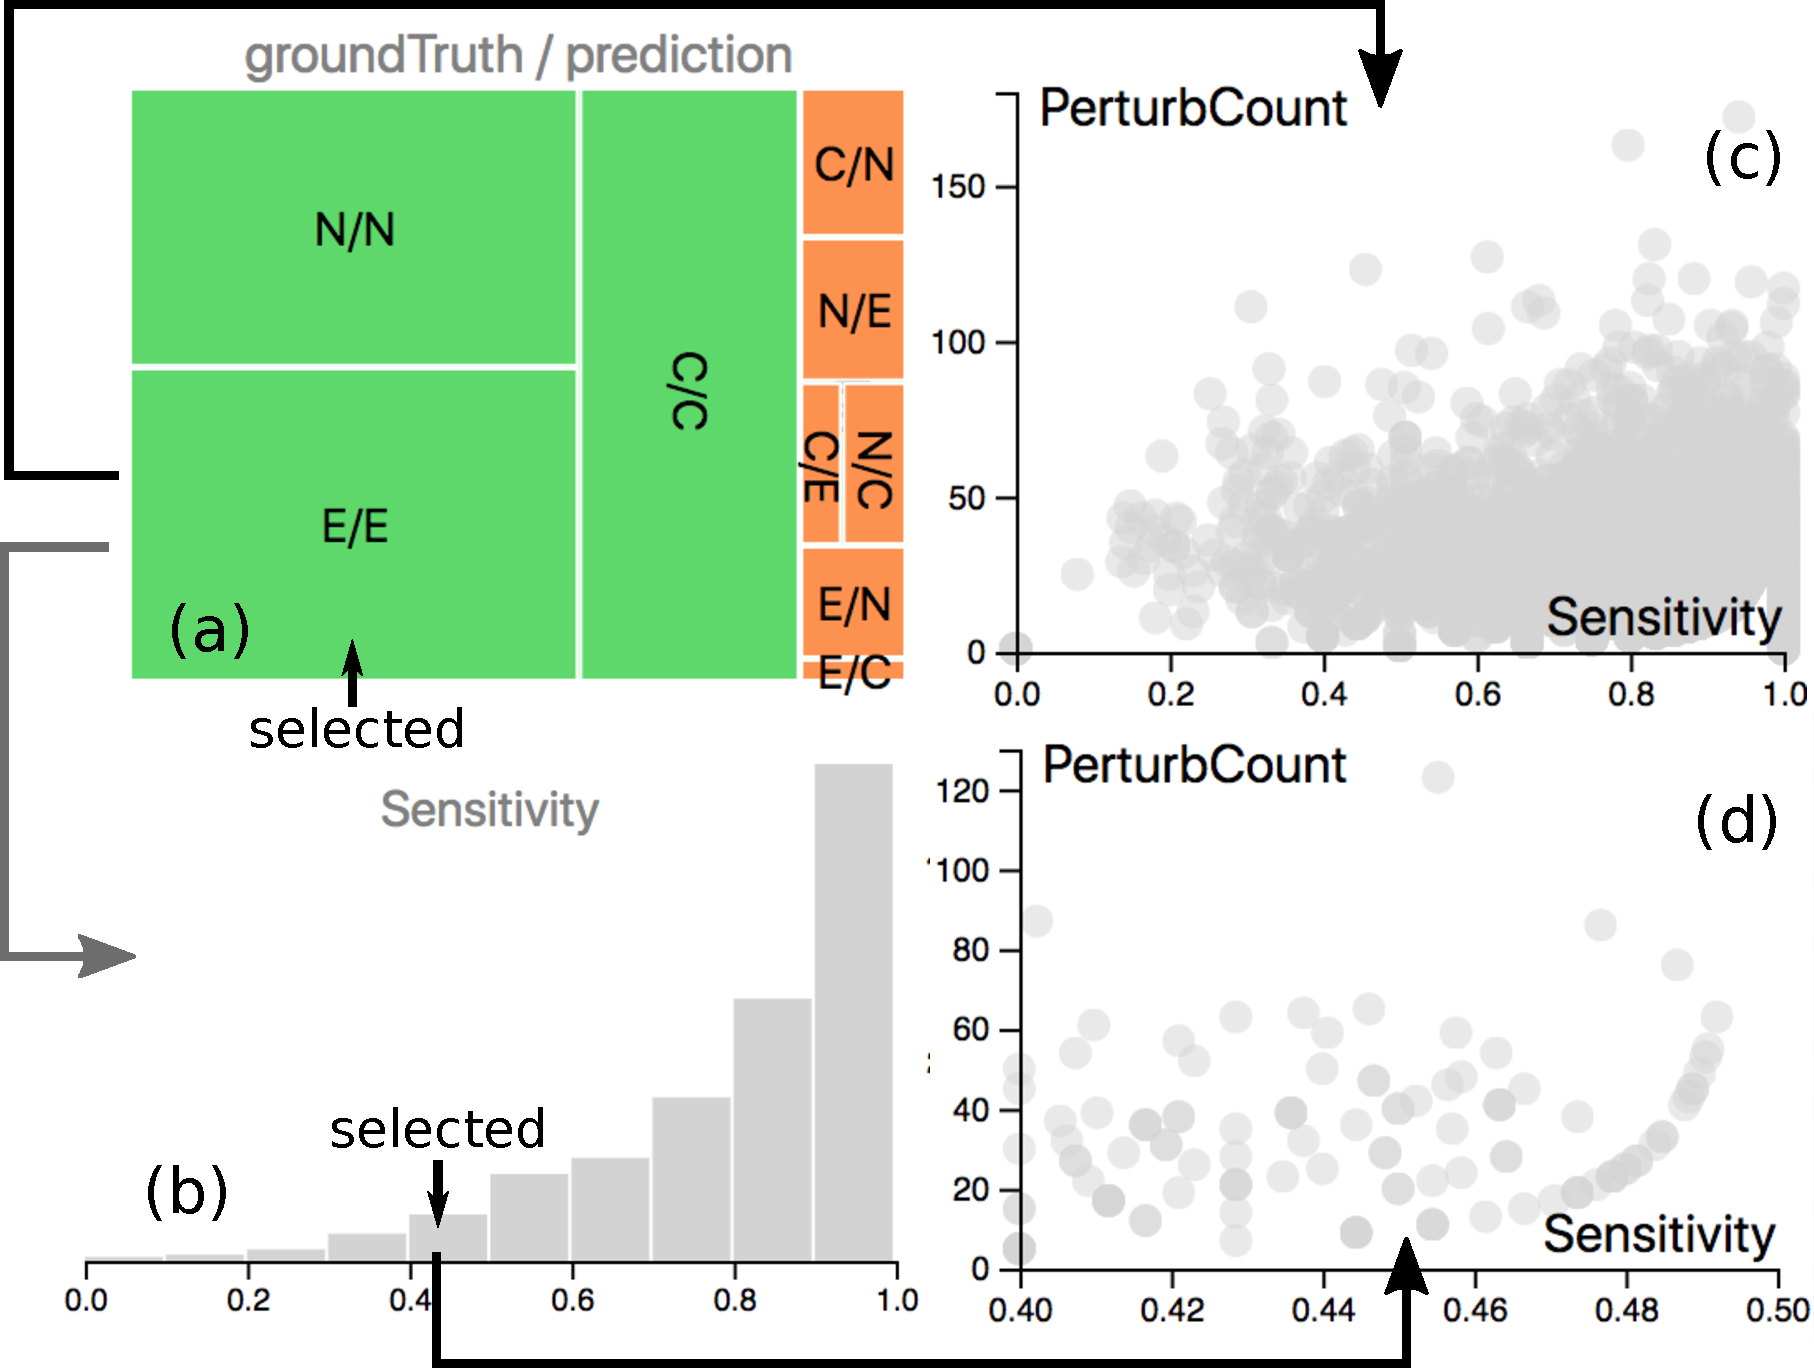
\includegraphics[width=1.0\linewidth]{summaryView}
 \vspace{-6mm}
 \caption{
%Summarize the prediction results and sensitivity of the entire development set, and provide an explorative interface to select an example of interest.
We summarized all prediction results of $10k$ sentence pairs in (a). The green block indicates correct predictions, the orange block indicates wrong predictions. %The tag on the node (e.g., E/E, E/N) encodes different types of the ground truth and the predicted label combinations (i.e., E/N is Entailment/Neural).
%
The user can click on a treemap node to focus on the specific type of scenarios (e.g., E/E, indicating both the ground truth and the predicted label are Entailment) to automatically reveal the histogram (b) and scatterplot (c) for displaying the selected subset.
%
The selection can be further narrowed down by selecting the bin in the histogram.
In (c) and (d), each point corresponds to one sentence pair.
 }
 \vspace{-2mm}
\label{fig:summaryView}
\end{figure}

To address these challenges, we introduce the summary view (see Fig.~\ref{fig:teaser}(a)), which consists of a treemap, a histogram, and a scatterplot, to summarize the prediction results of the $10k$ examples and provide the ability to drill down to individual examples for detailed analysis.
%treemap for prediction
As illustrated in Fig.~\ref{fig:summaryView}, we utilized a treemap (a) to encode the different combinations of the ground truth label and the predicted label. The green treemap blocks correspond to examples with correct predictions, whereas the orange blocks indicate failures. The size of the block encodes the number of examples belonging to each category.

By clicking on the treemap node, we can narrow down the selection by focusing on a specific scenario.
As we select the ``E/E'' (ground truth: E-Entailment / predicted label: E-Entailment) category in the treemap (see Fig.~\ref{fig:summaryView}(a)), the histogram (Fig.~\ref{fig:summaryView}(b)) and scatterplot  (Fig.~\ref{fig:summaryView}(c)) are shown. The histogram shows the distribution of the prediction stability in the selected category. For each example, the stability is defined by the ratio of the number of perturbed pairs with the same predicted label and the all the perturbed pairs. Assuming we have generated 100 pairs via the automated sentence perturbation operation (i.e., replace nouns and verbs with synonymous), the stability is 0.8 if 80 out of the 100 maintain the original label. 
%The \emph{stability} measures how likely a sentence pair will change its prediction after applying minor perturbations.% which helps the expert infer the model stability on the given example.
%
We can further narrow down the focused set by selecting the bins in the histogram (see Fig.~\ref{fig:summaryView}(b)).
%
In the scatterplot (Fig.~\ref{fig:summaryView}(c)(d)), each point corresponds to a sentence pair (the user can focus the rest of the visualization on one particular instance by selection). To help users better assess the \emph{stability} number, we also include the number of perturbed pairs (labeled as \emph{perturbCount}). If the \emph{perturbCount} is rather small ($<10$), then the \emph{stability} value is likely very noisy and unreliable. %For example, if the \emph{perturbCount} is rather small ($<10$), then the \emph{sensitivity} number is likely to be quite noisy and less trustworthy, as compared to the sensitivity ratio computed from a much larger number of perturbed pairs.



%The all pair
% \begin{itemize}
% \item How to go from 10k pair to one pair
% \item What constitute interesting example
% \item How to get a sense of overall prediction result
% \end{itemize}
